\chapter{Introduction to Deep Learning and Neural Architectures}
Let us now take a step back and think about the initial developments of artificial intelligence. Since their early days, AI-powered systems have been able to tackle and solve problems that had proven to be very difficult for humans, such as those that could be described by a list of formal and mathematical rules. The true challenge to artificial intelligence proved in fact to be solving tasks that are easy for people to perform, but hard for people to describe formally: problems that we solve intuitively, that feel automatic, like recognizing spoken words or faces in images. Several attempts were made to hard-code knowledge about the world in formal languages, but they were never able to achieve major successes.

Much of our knowledge is in fact based on \textbf{unstructured} inputs: computers then need to be able to capture this same knowledge and extract patterns from raw data, in order to behave in an intelligent way. \textbf{Machine learning} techniques can help in accomplishing this, enabling classification, clustering and rule discovery when given in input the right set of \textbf{features}. For many tasks, however, it is difficult to know which features should be extracted (like when recognizing objects in a photo, emotions from speech, etc.) and how information is structured and ``represented''. One solution to this problem is to use machine learning to discover not only the mapping from representation to output, but also the representation itself, with an approach known as \textbf{representation learning}. Learned representations often result in much better performance than the one that can be obtained by hand.

When designing features or algorithms for learning features, our goal is to separate the \textbf{factors of variation} that explain the observed data and that help in classification. These factors, unfortunately, are often quantities that cannot be directly observed but affect the ones that are observable, like in the case of \textbf{latent factors}. We then need to disentangle the factors of variation that allow us to complete our machine learning task successfully from the ones we do not care about (e.g., if we want to classify cars and trucks, the angle of the photo is not fundamental for classification purposes).

\section{Deep Learning}
\textbf{Deep learning} can address this problem of representation, learning by introducing representations that are expressed in terms of other, simpler representations. This allows computers to build complex concepts out of simpler ones. The quintessential example of a deep learning model is the \textbf{feedforward deep network} (also known as \textbf{multilayer perceptron}), which consists of a mathematical function mapping some set of input values to output values. An example can be seen in picture \ref{fig:ch6-innerworkingsofaffdn}:

\begin{figure}[hbt]
    \centering
    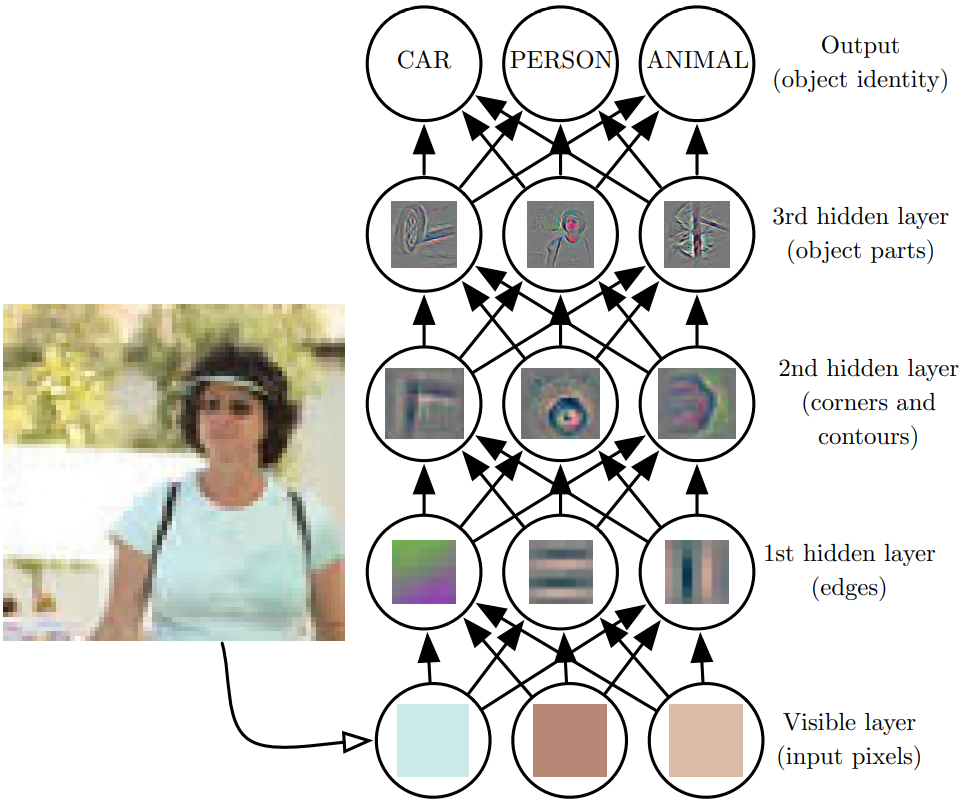
\includegraphics[scale=0.35]{Images/Chapter 6/ffdn-layers.png}
    \caption{Inner workings of a feedforward deep network}
    \source{Goodfellow et al. 2016}
    \label{fig:ch6-innerworkingsofaffdn}
\end{figure}

The idea of learning the right representation for the data provides one perspective on deep learning. A different one is that depth allows the computer to learn a multi-step computer program. Each layer of the representation can be thought of as the state of the computer’s memory after executing another set of instructions in parallel. Networks with greater depth can execute more instructions in sequence. Sequential instructions offer great power because later instructions can refer back to the results of previous ones.

The picture below sums up the differences between various types of artificial intelligence-based systems:

\begin{figure}[hbt]
    \centering
    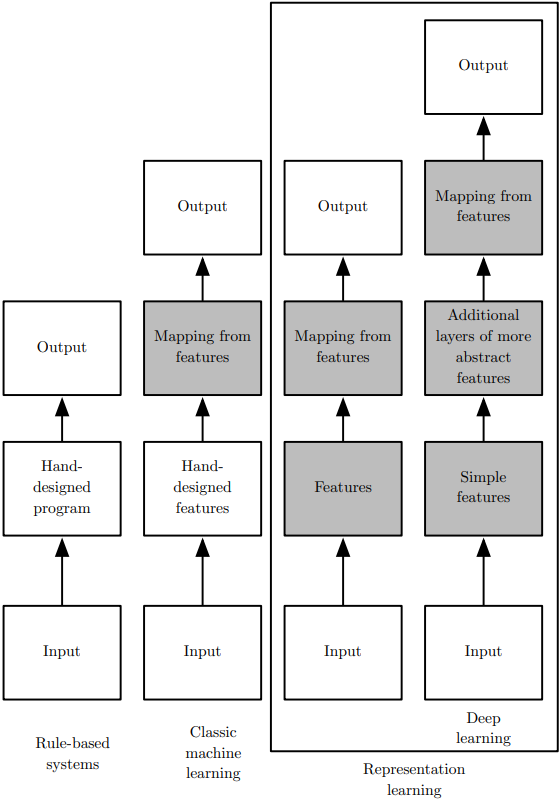
\includegraphics[scale=0.6]{Images/Chapter 6/types-ai.png}
    \caption{Differences between various types of AI-based systems}
    \source{Goodfellow et al. 2016}
    \label{fig:ch6-aitypesdifferences}
\end{figure}

\subsection{From theories of Biological Learning to Deep Learning}
Deep learning only \textit{appears} to be new due to its recent meteoric rise in popularity. As a matter of fact, instead, deep learning has been around since the 1940s, facing alternating periods of fervor and disappointment. There have been three main waves of development of deep learning:

\begin{itemize}
    \item Cybernetics (1940s-1960s).
    \item Connectionism (1980s-1990s).
    \item Deep learning (2006-today).
\end{itemize}

Let us now dive deeper into each of them.

\subsubsection{Cybernetics}
The origins of deep learning go by the name of ``cybernetics'', a term that became widespread thanks to Norbert Weiner’s book ``Cybernetics: control and communication in the animal and machine''. As we can imagine from this title, neuroscience was of great inspiration in this period: some of the earliest learning algorithms, in fact, were intended to be computational models of biological learning, attempting to reproduce what happens (or could happen) in the brain. The brain, in fact, provided a proof by example that intelligent behavior was possible, and a conceptually straightforward path to building intelligence seemed to be to reverse engineer the computational principles behind the brain and to duplicate its functionality. As a result, one of the names that deep learning has gone by is \textbf{artificial neural networks (ANNs)}. This school of thought led to the creation of simple linear models designed to take a set of $n$ input values $x_1,..., x_n$ and associate them with an output $y$. They would then learn a set of weights $w_1,...,w_n$ and compute the output $y=f(\boldsymbol{x},\boldsymbol{w})=x_1 w_1+...+x_n w_n$.

As a brief excursus and to understand the thought process that led to this formulation, we will now spend a few words describing what neurons are and how they work.

Neurons are electrically excitable cells that communicate with other cells via specialized connections called synapses. Communication consists of an all-or-nothing electrochemical pulse (of the same intensity each time the cell is stimulated) that takes place when the voltage of the neuron membrane changes by a large enough amount over a short interval. A typical neuron consists of a cell body (soma), dendrites and a single axon (the latter two being filaments that extrude from the soma) and can be seen in figure \ref{fig:ch6-multipolarneuron}.

\begin{figure}[hbt]
    \centering
    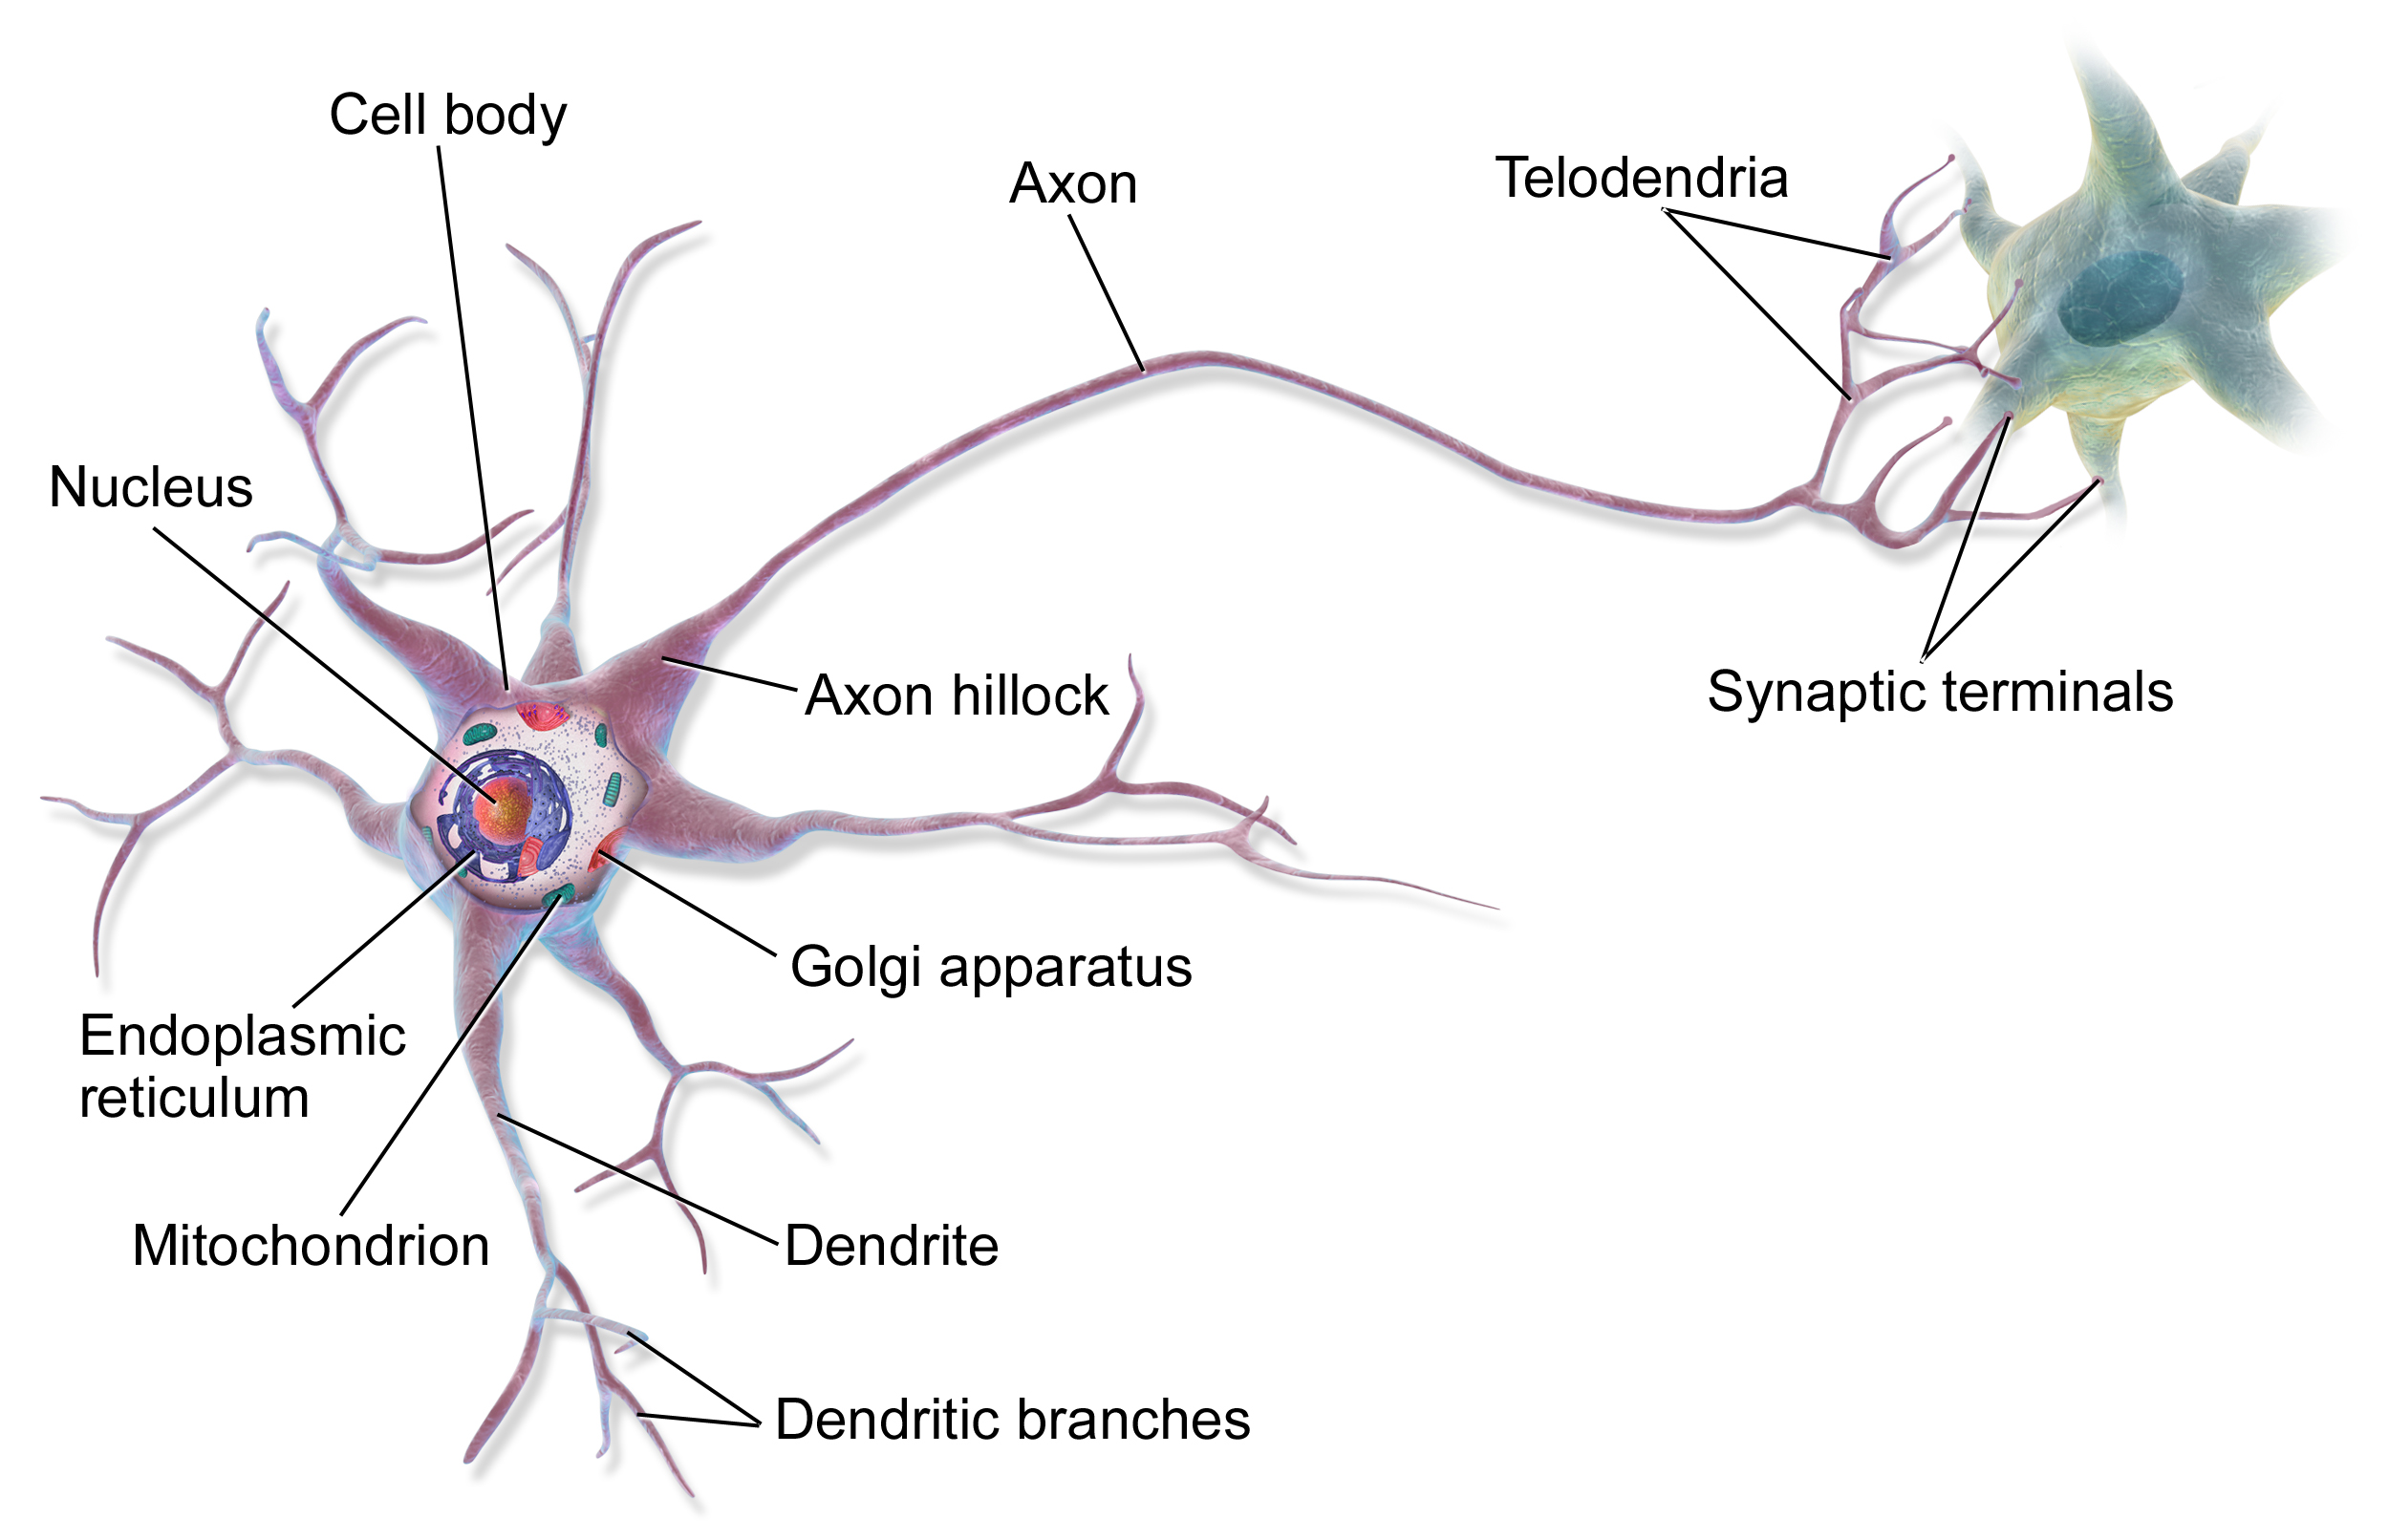
\includegraphics[scale=0.15]{Images/Chapter 6/multipolar neuron.png}
    \caption{Anatomy of a multipolar neuron.}
    \source{BruceBlaus on Wikipedia}
    \label{fig:ch6-multipolarneuron}
\end{figure}

Warren McCulloch (a neuroscientist) and Walter Pitts (a logician) studied the behavior of neurons and concluded that \textit{``Because of the ``all-or-none'' character of nervous activity, neural events and the relations among them can be treated by means of propositional logic''} \cite{MCCULLOCH199099}. In that article they also proposed a model of a simple artificial neuron which output 1 if the weighted sum of the inputs was above a certain threshold and 0 otherwise. Inputs could only have two values, 0 and 1, and be interpreted as \textit{excitatory} or \textit{inhibitory} according to their weights (+1 or -1). This model enabled operations such as \texttt{NOT} (one inhibitory input, with output threshold 0), \texttt{AND} ($n$ excitatory inputs with threshold $n$) and \texttt{OR} ($n$ excitatory inputs with threshold 1) by changing the weights of the inputs. A schema of their model can be found in figure \ref{fig:ch6-mccullochpittsartificialneuron}.

\begin{figure}
    \centering
    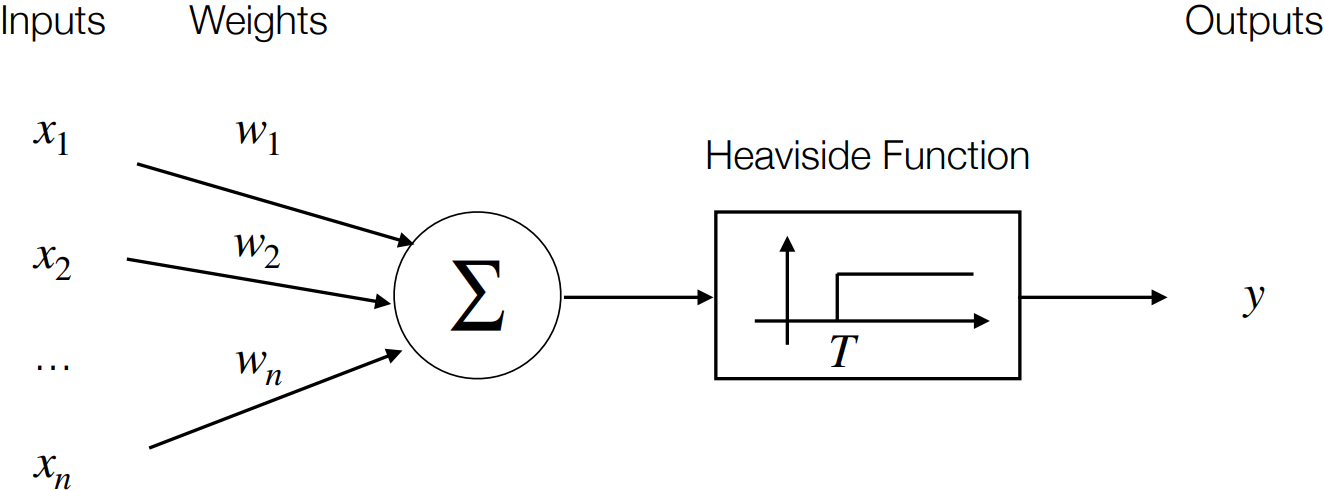
\includegraphics[scale=0.35]{Images/Chapter 6/mcculloch-pitts neuron.png}
    \caption{A schema of McCulloch and Pitt's artificial neuron.}
    \source{Prof. Mirco Musolesi}
    \label{fig:ch6-mccullochpittsartificialneuron}
\end{figure}

It is important to note that in their model the weights are \textbf{fixed} and must be set by a human operator. In 1949, though, the neuropsychologist Donald Hebb very importantly pointed out in his book “The Organization of Behavior” that \textit{``When an axon of cell A is near enough to excite a cell B and repeatedly or persistently takes part in firing it, some growth process or metabolic change takes place in one or both cells such that A’s efficiency, as one of the cells firing B, is increased''} \cite{10.1007/978-3-642-70911-1_15}. This means that synaptic connections are reinforced when two or more neurons are activated contiguously in time and space. In simpler words, ``Neurons that fire together, wire together'': the more we do something, the more ``habitual'' that learning will become. Hebb’s model led to the first simulations of artificial neural networks in the 1950s and can be seen in figure \ref{fig:ch6-hebbneuronmodel}.

\begin{figure}
    \centering
    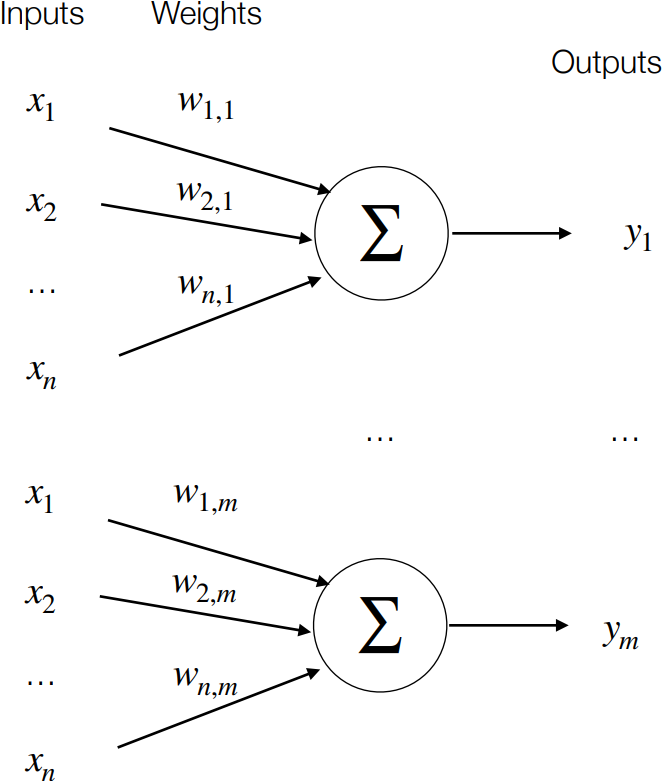
\includegraphics[scale=0.5]{Images/Chapter 6/hebb neuron model.png}
    \caption{Hebb's neuron model}
    \source{Prof. Mirco Musolesi}
    \label{fig:ch6-hebbneuronmodel}
\end{figure}

The Hebbian network model has a $n$-node input layer $\boldsymbol{x} = \left[x_1,x_2,...,x_n \right]^T$ and a $m$-node output layer $\boldsymbol{y} = \left[ y_1,y_2, ... ,y_m \right]^T$, with each output being the weighted sum of the corresponding inputs:

\begin{equation*}
    y_i = \sum_{j=1}^{n} w_{j,i} x_j 
\end{equation*}

The strengthening of the connections is represented by the following learning rule:

\begin{equation*}
    w_{j,i}^{new} \leftarrow w_{j,i}^{old} + \eta x_j y_i
\end{equation*}

Where $\eta$ is the \textbf{learning rate}. \emph{It must be noted that this model is different from the way current neural networks work}.

We had to wait until 1958, when Frank Rosenblatt created the \textbf{Perceptron} --a model for a machine that could learn the weights of different categories given examples of those categories-- for these ideas to be put into practice. 

Unfortunately, linear models such as the ones we just presented have many limitations (most famously, they cannot learn the \texttt{XOR} function) and this contributed to a period of disappointment and of little work on this field known as the “AI winter”.

\subsubsection{Connectionism}
The second wave of research on neural networks emerged in the 1980s primarily via a movement called \textbf{connectionism} or \textbf{parallel distributed processing}. Their core idea was that \textbf{many simple computational units could achieve intelligent behavior when networked together}. 

Several key concepts that arose from the connectionist movement remain central to today’s deep learning. Among these we find:

\begin{itemize}
    \item \textbf{Distributed representation}: each concept is not represented by a single neuron, but by a pattern of activation over a large number of neurons. The advantage of distributed representation is that when a small random subset of the network is altered it does not change the macroscopic behavior of the network. However, the disadvantage is that it is hard to interpret or modify the connection strength of the network by an outside observer.
    \item The \textbf{backpropagation algorithm} for training neural networks: the error obtained from the output layer is propagated backwards to the hidden layer and is used to guide training of the weights between the hidden layer and the input layer.
\end{itemize}

Another very important idea that can be found --along with the previous ones-- in a book titled ``Parallel Distributed Processing'' is that of ``Learning and Relearning in Boltzmann Machines'' \cite{10.5555/104279.104291}. A Boltzmann Machine is a network of symmetrically connected, neuron-like units that make stochastic decisions about whether to be on or off based on the data fed to the network while training. We consider two types of Boltzmann Machines, which we can also see in figure \ref{fig:ch6-boltzmannmachines}:

\begin{figure}
    \centering
    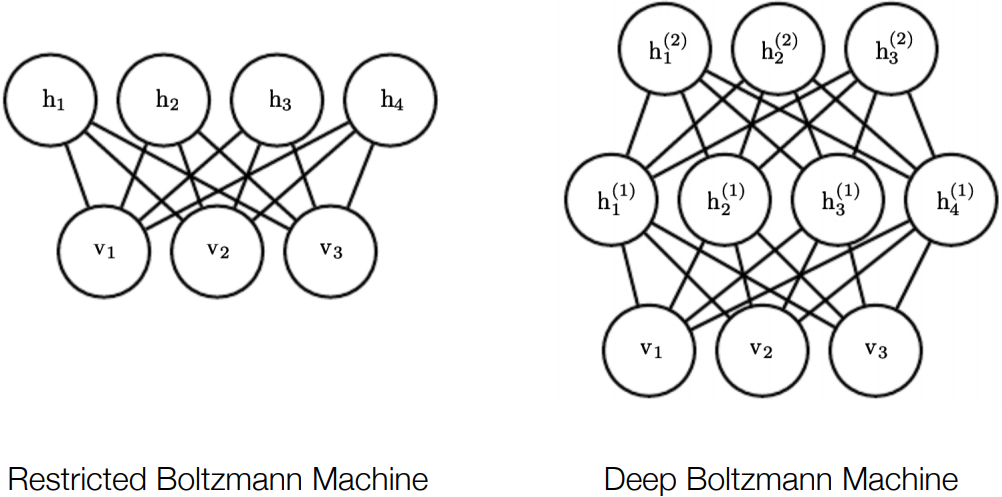
\includegraphics[scale=0.5]{Images/Chapter 6/boltzmann machines.png}
    \caption{Boltzmann machines}
    \source{Goodfellow et al. 2016}
    \label{fig:ch6-boltzmannmachines}
\end{figure}

\begin{itemize}
    \item \textbf{Restricted Boltzmann Machines}, made up of an input and a hidden layer. In this machine neurons must form a bipartite graph\footnote{A graph whose vertices can be divided into two disjoint and independent sets $U$ and $V$ such that every edge connects a vertex in $U$ to one in $V$, see \url{https://en.wikipedia.org/wiki/Bipartite_graph}}.
    \item \textbf{Deep Boltzmann Machines} in which there may be multiple hidden layers, with hidden nodes connected to each other.
\end{itemize}

Note that, unlike most neural networks, the connections are bidirectional and there is no output layer. The training phase for this network leverages the bidirectionality, as it allows for a continuous feedback loop between the input and the hidden layer that is bound to eventually stabilize, allowing the determination of the connection weights. The lack of an output layer is instead explained by the generative nature of these networks: if we give them a partial input (like a section of an image), the network will generate the missing parts, effectively making the results appear in the input layer.

\subsection{Second AI winter and the current AI summer}
The amount of progress being made at the time led to the creation of unrealistic expectations that, once they could not be met, brought in a second AI winter that lasted until the mid-1990s.

The current AI summer, instead, started in 2006, when Geoffrey Hinton and Simon Osindero proposed ``A fast learning algorithm for deep belief nets''  \cite{10.1162/neco.2006.18.7.1527} (with a strategy called \textit{greedy layer-wise pre-training}) that enabled fast training even for networks with high dimensionality.

This breakthrough opened up a myriad of new possibilities for deep learning. Nowadays, in fact, deep learning applications are aplenty: 

\begin{itemize}
    \item Computer vision.
    \item Machine translation.
    \item Speech generation.
    \item Protein folding.
    \item ...
\end{itemize}

One of deep learning's biggest achievements (and the more relevant one for us) has been its extension to the field of reinforcement learning, enabling what is now known as \textbf{deep reinforcement learning}.

\section{Deep Neural Networks}
After a general overview of the history of deep learning, we now move on to more practical details about how deep neural networks work. Let us start by looking at the structure of a modern neural network and the corresponding schematized version we will use in this course (figure \ref{fig:ch6-dnnandschema}).

\begin{figure}[h]
    \hfill
    \subfigure[]{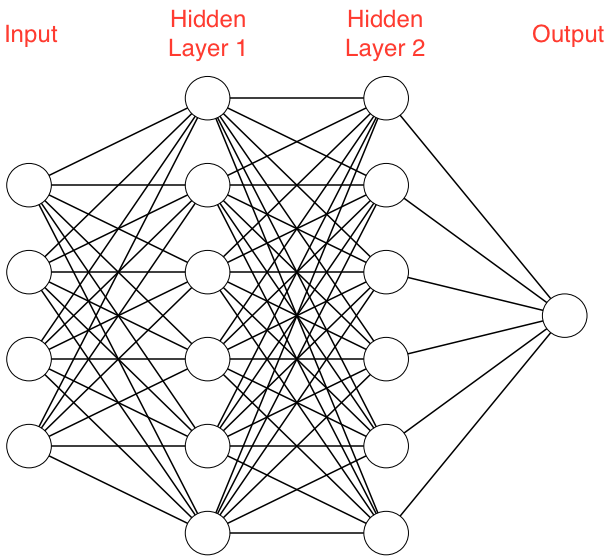
\includegraphics[width=5cm]{Images/Chapter 6/deep_neural_network.png}}
    \hfill
    \subfigure[]{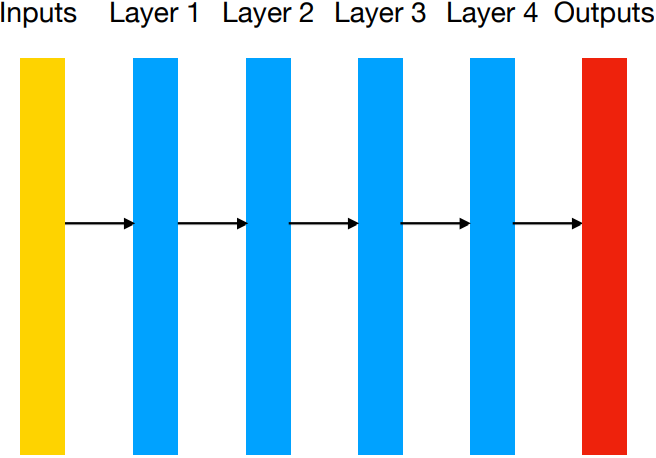
\includegraphics[width=5cm]{Images/Chapter 6/dnn notation.png}}
    \hfill
    \caption{(a) A modern deep neural network and (b) the simplified notation we will use in this course}
    \source{(a) andrewkruger on GitHub, (b) prof. Mirco Musolesi}
    \label{fig:ch6-dnnandschema}
\end{figure}

These types of networks are known as \textbf{deep feedforward networks} or \textbf{multilayer perceptrons (MLP)} and are the quintessential deep learning models. Their goal is to approximate some function $f^*$: for example, for a classifier, $y=f^* (\boldsymbol{x})$ maps an input $\boldsymbol{x}$ to a category $y$. A feedforward network defines a mapping $y=f(\boldsymbol{x},\boldsymbol{\theta})$ and learns the value of the parameters $\boldsymbol{\theta}$ that result in the best function approximation. This is done by feeding the network some training data and comparing our estimates to the true labels by means of a \textbf{loss function}. The \textbf{loss scores} thus obtained, will then be given to an \textbf{optimizer} which will update the weights, as we can see from figure \ref{fig:ch6-lossoptimizationdnn}.

\begin{figure}[hp]
    \centering
    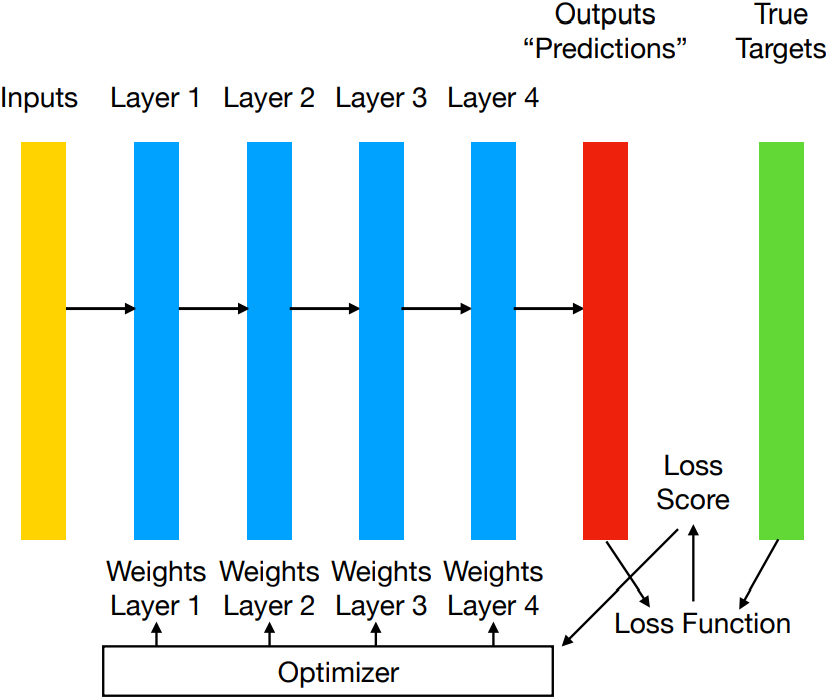
\includegraphics[scale=0.5]{Images/Chapter 6/dnn-loss-optimizer.png}
    \caption{Loss scores optimization in a DNN}
    \source{Prof. Mirco Musolesi}
    \label{fig:ch6-lossoptimizationdnn}
\end{figure}

Each neuron (also referred to as unit or node) of the network will then be as shown in figure \ref{fig:ch6-dnnunit}.

\begin{figure}[hp]
    \centering
    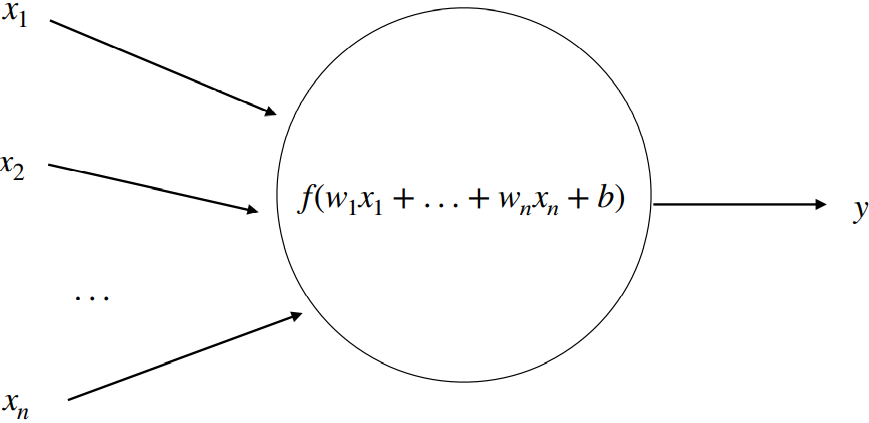
\includegraphics[scale=0.5]{Images/Chapter 6/dnn-unit.png}
    \caption{A neuron of a DNN}
    \source{Prof. Mirco Musolesi}
    \label{fig:ch6-dnnunit}
\end{figure}

Where $f$ is the activation function, a nonlinear combination of the inputs and the weights, and $b$ is the \textbf{bias}, a fixed, (typically) random value that works as ``noise'' for the network and that helps in avoiding suboptimal solutions.

There are many activation functions, with various characteristics and properties. Among the most common ones\footnote{For a more comprehensive list of activation functions, see \url{https://en.wikipedia.org/wiki/Activation_function}.} we find:

\begin{itemize}
    \item \textbf{Rectified Linear Unit (RELU)}: given the value $z$ in input, it returns $\max(0,z)$.
    \item \textbf{Logistic sigmoid}: given the value $z$ in input, it returns $\frac{1}{1+e^z}$.
    \item \textbf{Arctan}: given the value $z$ in input, it returns $\tan^{-1}z$.
    \item \textbf{Softmax}: given a vector of real numbers in input $\boldsymbol{z}$ of dimension $n$, the softmax function normalizes it into a probability distribution consisting of $n$ probabilities proportional to the exponential of each element $z_i$ of the vector $\boldsymbol{z}$.
\end{itemize}

It is very important to note that, while the RELU function, the logistic sigmoid and the arctangent only receive in input (and output) a single real value, \textbf{the softmax function receives in input a vector of real numbers, and outputs a vector of the same dimension}. This is particularly useful for the output layer of our network in classification problems: we can use one of the 1-dimensional activation functions in the hidden layers and use the softmax function to output probabilities\footnote{We say that these probabilities are uncalibrated: until we calibrate them, they do not represent actual probabilities, they are only monotonically ordered from less to more likely.} of the input belonging to one of the $n$ classes of our classification problem. Formally, the softmax function is defined as such:

\begin{equation}
    \text{softmax}(\boldsymbol{z})_i= \frac{e^{z_i}}{\sum_{j=1}^{n} e^{z_j}} \  \text{for } i = 1, ..., n
\end{equation}

\subsection{Gradient-based optimization}
After seeing a handful of activation functions that allow our networks to work and to produce outputs, we can now focus on another very important piece of the puzzle: the optimizer.

As we saw before, each neural layer transforms its input by applying a function as follows:

\begin{equation*}
    output = f(w_1 x_1 + ... + w_n x_n + b)
\end{equation*}

The learning is predicated on the gradual adjustment of the weights based on a feedback signal (typically the \textbf{loss function}, also called \textbf{cost function} or \textbf{error function}) and can be summed up in the following steps:

\begin{enumerate}
    \item Draw a batch of training examples $\boldsymbol{x}$ and their corresponding targets $\boldsymbol{y}_{target}$.
    \item Run the network on $\boldsymbol{x}$ (forward pass) to obtain the predictions $\boldsymbol{y}_{pred}$.
    \item Compute the loss of the network on the batch (a measure of the mismatch between $\boldsymbol{y}_{pred}$ and $\boldsymbol{y}_{target}$).
    \item Update all the weights of the network in a way that it reduces the loss of this batch. By working in terms of batches, we avoid overfitting to a single example. 
\end{enumerate}

Given a differentiable function, the last step can be performed by means of \textbf{gradient descent} as shown in figure \ref{fig:ch6-gradientdescent}, even analytically if the number of weights is particularly small.

\begin{figure}[hb]
    \centering
    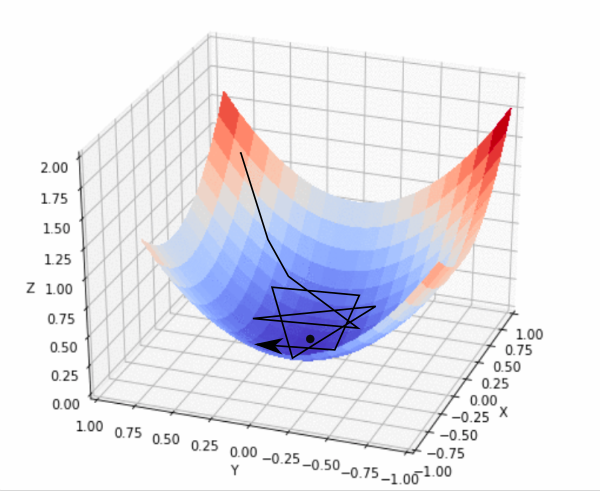
\includegraphics[scale=0.15]{Images/Chapter 6/gradient-descent.png}
    \caption{Gradient descent in a 3-dimensional space.}
    \source{Ayoosh Kathuria on PaperSpace}
    \label{fig:ch6-gradientdescent}
\end{figure}

This, however, is almost never the case, making it necessary to use approximate methods. Gradient descent methods follow the blueprint just presented, and update the weights by moving the parameters in the opposite direction of the gradient as follows:

\begin{enumerate}
    \item Draw a batch of training examples $\boldsymbol{x}$ and their corresponding targets $\boldsymbol{y}_{target}$.
    \item Run the network on $\boldsymbol{x}$ (forward pass) to obtain the predictions $\boldsymbol{y}_{pred}$.
    \item Compute the loss of the network on the batch (a measure of the mismatch between $\boldsymbol{y}_{pred}$ and $\boldsymbol{y}_{target}$).
    \item Compute the gradient of the loss function with regards to the network’s parameters (backward pass). \item Move the parameters in the opposite direction of the gradient with:
    
        \begin{itemize}
            \item $w_j \leftarrow w_j + \Delta w_j = w_j - \eta \frac{\partial J}{\partial w_j}$ for a single piece of data at a time.
            \item $w_j \leftarrow w_j + \Delta w_j = w_j - \eta\ \text{average} \left( \frac{\partial J}{\partial w_j} \right)$ for batches of $k$ samples.
        \end{itemize}
        
        Where $J$ is the loss function.
\end{enumerate}

If the input is drawn randomly from the available data, we refer to this as \textbf{Stochastic Gradient Descent}. If we use batches of data selected randomly, we call it \textbf{(mini)-batch Stochastic Gradient Descent}. It is also important to note that this is a simplified model, where we assume only one layer (and thus only one loss function): if this was not the case, we would have to calculate the gradients of all the loss functions and apply the weight correction to all the layers. A more realistic visualization of the ``landscape'' that we have to traverse during gradient descent is shown in figure \ref{fig:ch6-losslandscape}.

\begin{figure}[htb]
    \centering
    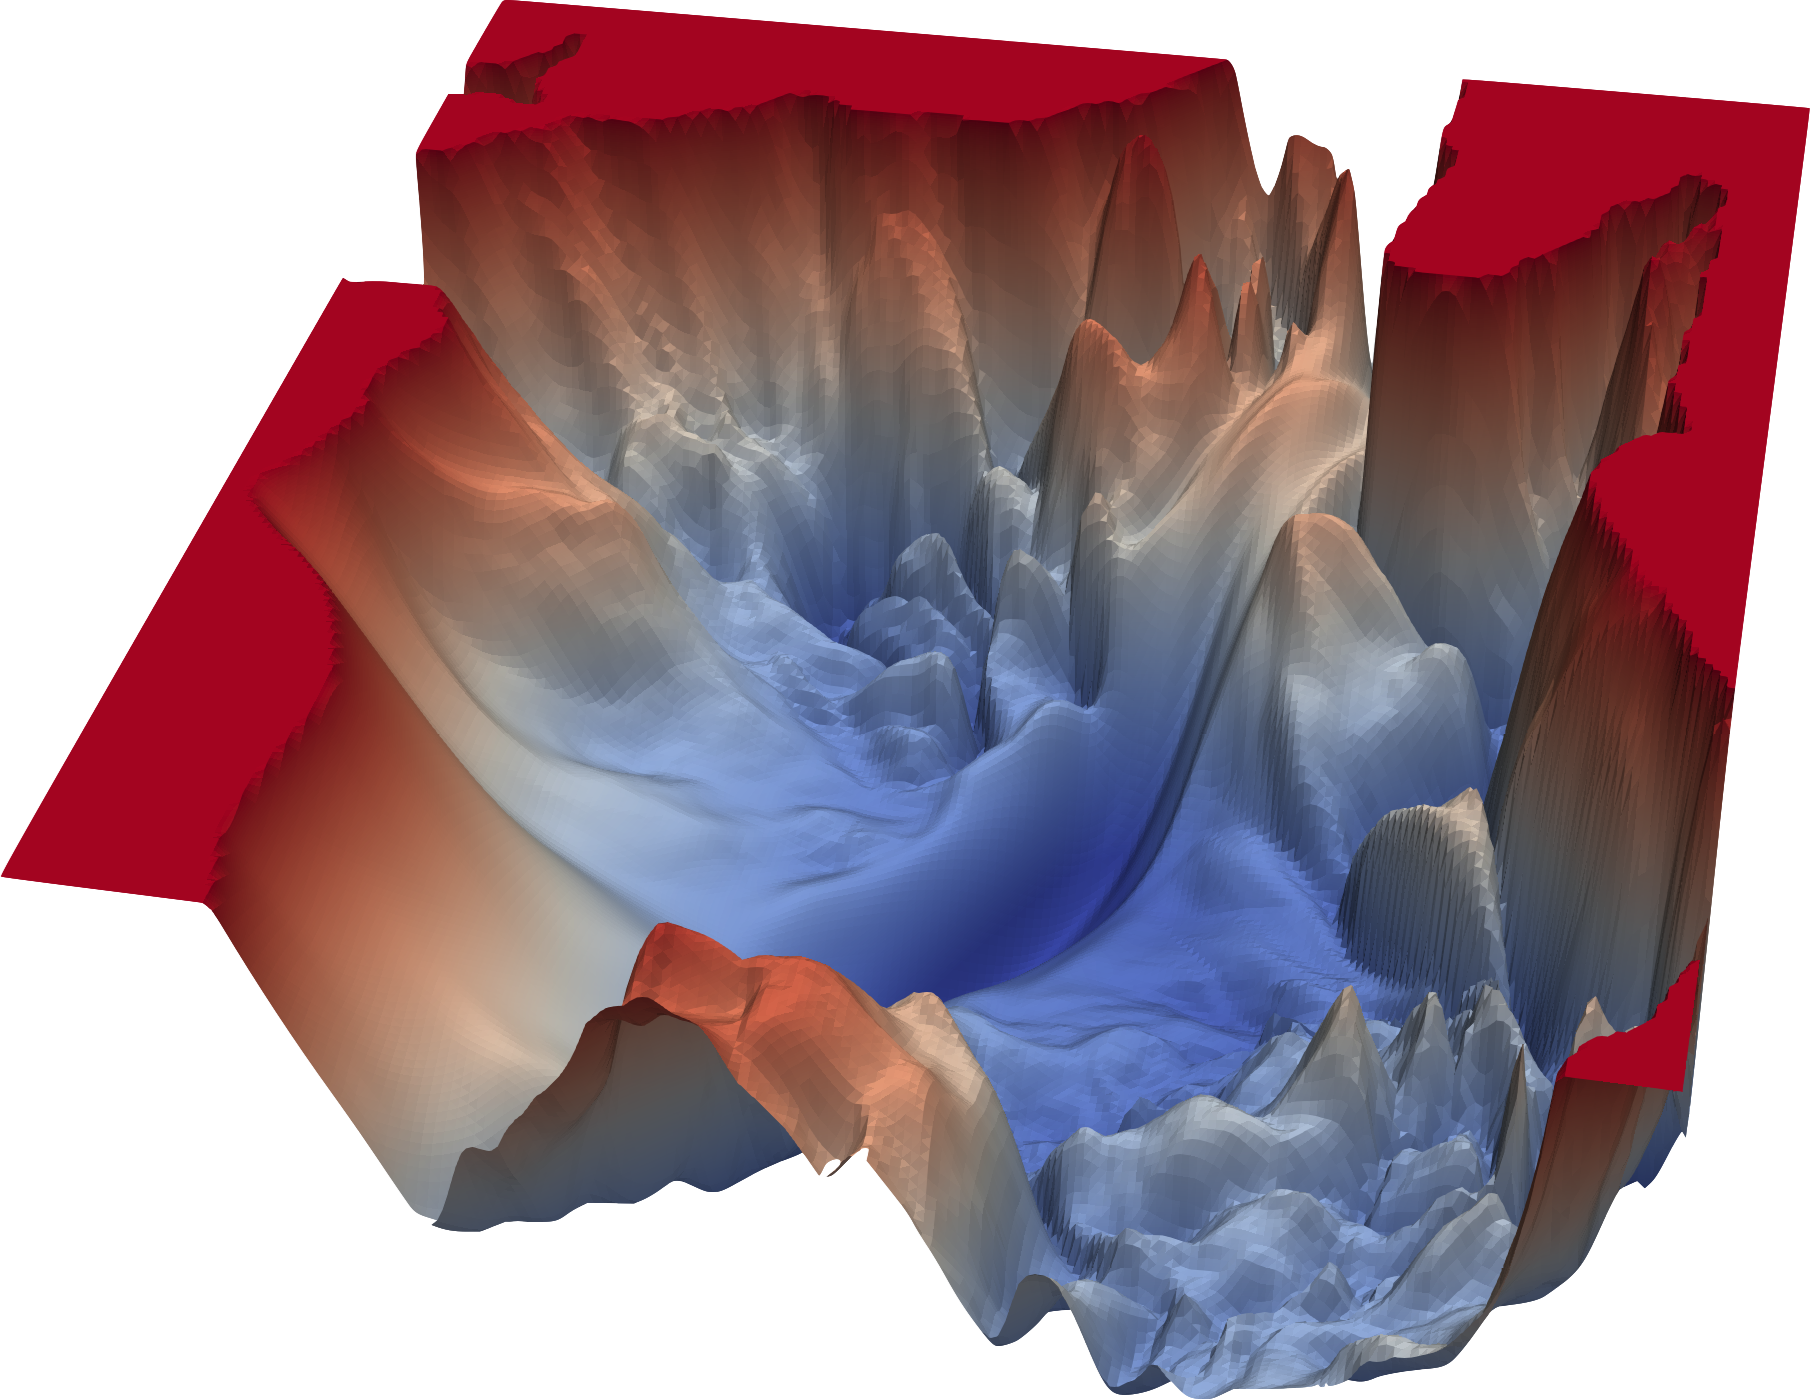
\includegraphics[scale=0.15]{Images/Chapter 6/landscape.png}
    \caption{The loss landscape of a neural network.}
    \source{University of Maryland}
    \label{fig:ch6-losslandscape}
\end{figure}

\subsection{The backpropagation algorithm}
Now that we have seen how to perform weight optimization, we briefly introduce the \textbf{backpropagation algorithm}, a method through which we can apply this correction.

Let us imagine we have a network with $L$ layers, each with a set of weights represented by the vector $\boldsymbol{W}^l$, with $l$ being the layer we are considering. The network output will be then given by:

\begin{equation}
    \boldsymbol{y}_{pred} = f^L \Bigg(\boldsymbol{W}^L \Big(f^{L-1} \big(\boldsymbol{W}^{L-1} ... f^1 \left(\boldsymbol{W}^1 \boldsymbol{x}\right) ...\big)\Big)\Bigg)
    \label{eq:ch6-nnoutput}
\end{equation}

To perform the update, we can apply the chain rule (shown here) to calculate the derivative of the composite function represented by our network as such:

\begin{equation*}
    \frac{d}{dx} \Big[ f \big( g(x) \big) \Big] = f' \big( g(x) \big) g' (x)
\end{equation*}

It is called backpropagation algorithm because it starts by calculating the gradient of the final loss value and works backwards from the right-most layers to the left-most ones, applying the chain rule to compute the contribution that each weight had in the loss value.